eн вызов специалиста, который средствами микроконтроллера извлечёт необходимую информацию.\chapter{Технический проект}
	\section{Техническое описание}
		\subsection{Назначение}
				Устройство предназначения для мониторинга и включения системы оповещения в случае
			реагирования датчиков движения.
		\subsection{Принцип работы}
				К выходам АЦП подключаются датчики движения. К выходу ЦАП подключается
			управляющее устройство, компаратор.

				Сигналы, полученные от датчиков, поступают на аналоговый сумматор AD1, значение
			выхода (контакт 6) AD1 преобразуется в цифровой сигнал с помощью DD1. К
			управляющему устройству DD4 подключаются выходs с преобразователя DD1 и с микроконтроллера
			DD3. Результат сравнения получаемой и хранимой информации подаётся с управляющего
			устройства DD4 на преобразователь DD2. Сигналы, полученные от DD2 выводится на диоды
			R1-R10. Необходимые настройки хранятся в микроконтроллере DD3.

				Настройки, определяемые производителем, устанавливаются с помощью X1, выходы
			которого подключены к микроконтроллеру DD3.
	\section{Расчёты}
			Прибор сравнивает значение с датчиков и заданное значение, результаты передаются на
		выходы управляющего устройства.

			Различные варианты реализации представлены на рисунках ниже
		\subsection{Оценка теплового режима}
				Тепловой режим выбирается с помощью диаграммы, приведенной на рисунке \ref{projectp1}. Область
			разделяемой зоны соответствует каждому способу охлаждения
			\begin{figure}[ht!]
				\centering
				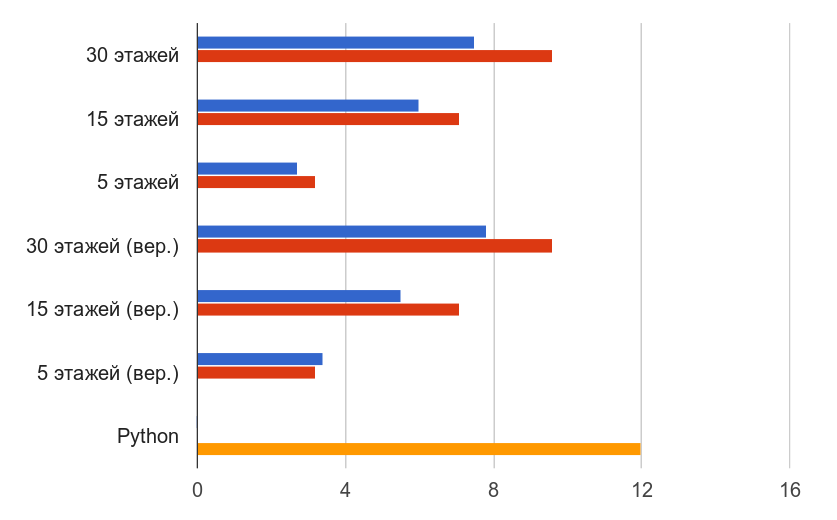
\includegraphics[width=50mm]{src/pictures/projectp1.png}
				\caption{Диаграмма выбор способа охлаждения}\label{projectp1}
			\end{figure}
			\begin{enumerate}
				\item Естественное;
				\item Естественное или принудительная конвекция;
				\item Принудительная конвекция;
				\item Принудительная конвекция или принудительная жидкостная.
			\end{enumerate}
			\subsubsection{Допустимый перегрев нагретой зоны}
					Для определения зоны необходимо рассчитать $\bigtriangleup T_{oc}$(допустимый перегрев нагретой зоны): \\
				$\bigtriangleup T_{oc} = T_{min} - T_{oc}$
				, где $T_{min}$ – допустимая температура нагретой зоны,
				$T_{oc}$ – максимальная температура окружающей среды.

					Расчет поверхности нагретой зоны \\
				$S_k = 2 * (L_1 * L_2 + (L_1 + L_2) * L_3 * K_3)$
				, где $L_1$ – длина, м; $L_1 = 0,12$
				, $L_2$ – ширина, м; $L_2 = 0,09$
				, $L_3$ – высота, м; $L_3 = 0,05$
				, $K_3$ – коэффициент заполнения, равный отношению объема функциональных и монтажных элементов внутри объема корпуса к его внутреннему объему.
			\subsubsection{Плотность теплового потока}
				$q = {P * K}/{S_k}$
				, где Кn = 1 при н.у. (760 мм. рт.ст);Р – суммарная тепловая мощность.
			\subsubsection{Расчет}
				$\bigtriangleup T_{oc} = 70 - 35 = 35$ \\
				$S_k = 2 * (0,12 * 0,09 + (0,12 + 0,09) * 0,05 * 0,0116) = 0,0214 \textup{м}^2$ \\
				$q = {4}/0,0214 = 201,34$ $\textup{Вт/м}^2$ \\
				$lg(201,34) = 2,3$ $\textup{Вт/м}^2$

				Из полученных расчетов можно сделать вывод, что прибору не требуется дополнительное охлаждение.
		\subsection{Расчет надежности}
			Для расчета средней наработки на отказ используется формула 4 и данные из таблицы \ref{projectt1}, полученные из справочника.
			$T_{cp} = 1/{\Sigma\lambda_i}$, 
			$T_{cp} = 366300$ часов.
			{
\changefontsizes[12pt]{12pt}
\captionsetup{font=large,margin=21pt}

\vspace{14pt}
\begin{longtable}[t]{@{\extracolsep{\fill}}|l|@{\hskip+35pt}p{0.15\textwidth}|@{\hskip+35pt}p{0.15\textwidth}|@{\hskip+35pt}p{0.15\textwidth}|}
% \begin{longtable}[t]{@{\extracolsep{\fill}}|l|@{\hskip-28pt}c|@{\hskip-28pt}c|@{\hskip-28pt}c|}
	\caption{Сравнение по среднему времени ожидания \vspace{-35pt}} \label{projectt1} \\ \hline
			&&&\\[-7pt]
	Способ управления
		& 30 этажей \hspace{14pt}
			& 15 этажей \hspace{14pt}
				& 5 этажей  \hspace{14pt}  \\  \hline
	\endfirsthead
	\caption* {Продолжение таблицы \ref{projectt1}\vspace{-35pt}}\\ \hline
			&&&\\[-7pt]
	Способ управления
		& 30 этажей
			& 15 этажей
			& 5 этажей   \\ \hline \endhead 
			&&&\\[-7pt]
	I тип     &	7.5		&	6	& 2.7	\\ \hline
			&&&\\[-7pt]
	II тип    &	9.6		&	7.1	& 3.2		\\ \hline
\end{longtable}
}

		\subsection{Программная часть}
			\subsubsection{Описание}
				Программа, ккоторая вшивается в микроконтроллер, работает по приципу автомата. То есть при послуплении новой информации вся хранимая информация сдвикается на определённый размер записи. В момент переполнения банка данных самая старая запись стирается и записывается новая в начало, а остальные записи так же сдвигаются на размер записей. 
				
				Запись имеет следующий формат: <<HH:MM dd.mm.yyyy>>. 
				
				При необходимости считывания записией, нужeн вызов специалиста, который средствами микроконтроллера извлечёт необходимую информацию.
			\subsubsection{Кодирование}
				На рисунке \ref{projectp2} изабражен листинг проживки микроконтроллера.
				\begin{figure}[ht!]
					\centering
					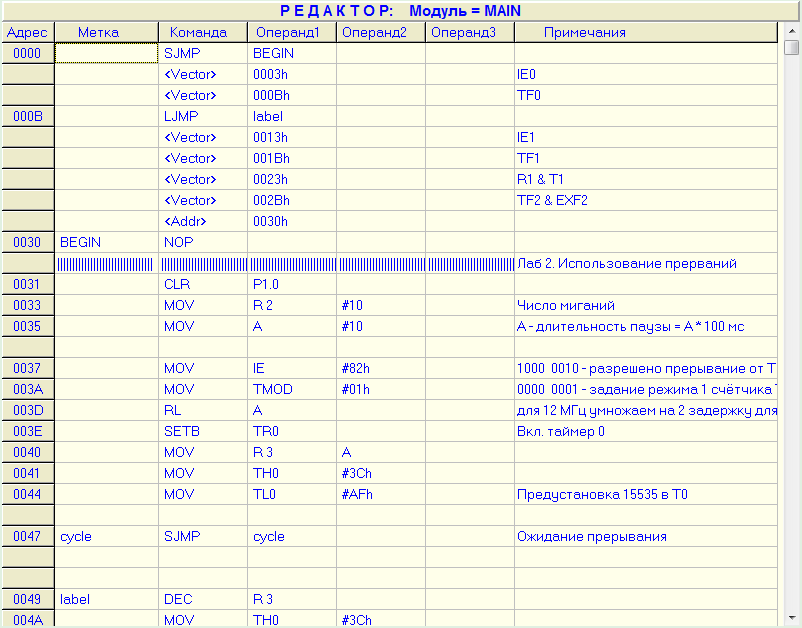
\includegraphics[width=150mm]{src/pictures/program.png}
					\caption{Диаграмма выбор способа охлаждения}\label{projectp2}
				\end{figure}
